\documentclass[notheorems, handout]{beamer}

\usetheme[numbers,totalnumbers,compress, nologo]{Statmod}
\usefonttheme[onlymath]{serif}
\setbeamertemplate{navigation symbols}{}
\setbeamertemplate{theorems}[numbered]
\setbeamertemplate{caption}[numbered]

\mode<handout> {
	\usepackage{pgfpages}
	\setbeameroption{show notes}
	\setbeamercolor{note page}{bg=white}
	\setbeamercolor{note title}{bg=gray!10}
	\setbeamercolor{note date}{fg=gray!10}
}

\usepackage[utf8x]{inputenc}
\usepackage[T2A]{fontenc}
\usepackage[russian]{babel}
\usepackage{tikz}
\usepackage{ragged2e}
\usepackage{amsmath,amssymb}
\usepackage{graphicx}
\usepackage{caption}
\usepackage{subcaption}
\usepackage{color}
\usepackage{dcolumn}
\usepackage{bm}
\usepackage{float}
\usepackage{csquotes}
\usepackage[backend=biber, style=authoryear, sorting=nyt]{biblatex} % Используем biblatex
\addbibresource{ref.bib} % Имя файла с библиографией
\usepackage{xcolor}

\newtheorem{corollary}{Следствие}
\newtheorem{theorem}{Теорема}
\newtheorem{remark}{Замечание}
\newtheorem{comment}{Замечание}
\newtheorem{lemma}{Лемма}
\newtheorem{sentence}{Предложение}
\newtheorem{definition}{Определение}
\newtheorem{formulation}{Формулировка}
\newtheorem{statement}{Постановка}
\DeclareMathOperator{\R}{\mathbb{R}}
\DeclareMathOperator{\rank}{\mathrm{rank}}
\newcommand{\norm}[1]{\left\|#1\right\|}

\newcommand{\SSA}{\textbf{SSA}}
\newcommand{\GSSA}{\textbf{GSSA}}
\newcommand{\CISSA}{\textbf{CiSSA}}
\newcommand{\TS}{\mathsf{X}}

\newcommand{\MSE}{\operatorname{MSE}}


\title[Модификации метода $\SSA$]{Модификации метода анализа сингулярного спектра для анализа временных рядов: Circulant SSA и Generalized SSA }

\author{Погребников Н. В., гр. 21.Б04-мм}

\institute[Санкт-Петербургский Государственный Университет]{%
	\small
	Санкт-Петербургский государственный университет\\
	Прикладная математика и информатика\\
	Вычислительная стохастика и статистические модели\\
	\vspace{1cm}
%	4 курс (бак.) <<Производственная практика (научно-исследовательская работа)>>\\(Семестр 6)
	Научный руководитель:  д. ф.-м. н., доц. Голяндина Н. Э.
}
	

\date[Зачет]{Санкт-Петербург, 2025}

\subject{Talks}

\begin{document}

	\begin{frame}[plain]
		\titlepage
		
		% \note{Научный руководитель  д.\,ф.-м.\,н., доц. Голяндина Нина Эдуардовна,\\
		% 	кафедра статистического моделирования}
	\end{frame}
	
	%\section{Короткая тема}
	%\subsection{Общие слова}
	
%	\setbeameroption{show notes}
	
	\begin{frame}{Введение}
		Пусть $\TS = (x_1, \dots, x_{N})$ -- временной ряд длины \( N \), \( x_i \in \mathbb{R} \) -- наблюдение в момент времени \( i \).

		\(\TS = \TS_{\text{Trend}} + \TS_{\text{Periodics}} + \TS_{\text{Noise}}\), где:
		\begin{itemize}
			\item \( \TS_{\text{Trend}} \) -- тренд, медленно меняющаяся компонента;
			\item \( \TS_{\text{Periodics}} \) -- сумма периодических компонент;
			\item \( \TS_{\text{Noise}} \) -- шум, случайная составляющая.
		\end{itemize}

		\textbf{\structure{Методы}:}
		$\SSA$ -- метод, позволяющий раскладывать временной ряда в сумму интерпретируемых компонент \parencite{golyandina2001analysis}; 
		$\GSSA$ -- модификация $\SSA$ на основе добавления весов \parencite{gu2024generalized}; 
		$\CISSA$ -- модификация $\CISSA$ на основе циркулярной матрицы \parencite{bogalo2020}.

		\textbf{\structure{Задача}:} 
		Описание модификаций в контексте теории $\SSA$, сравнение алгоритмов, реализация их на языке R.
		
		% \note{
		% 	\textcolor{red}{\textbf{TODO}} Дописать ссылки
		% 	}
	\end{frame}

	\begin{frame}{По чему будем сравнивать?}
		% \textcolor{red}{\textbf{TODO}} Оформить слайд

		\textbf{\structure{Пример}} 
		$\TS = \TS_{1} + \TS_{2} + \TS_{\mathrm{Noise}}=e^{A{n}}
		\sin\left({2\pi\omega_1 n}\right) + 
		\cos\left({2\pi\omega_2 n}\right) + \varepsilon_n$.

		$\omega_1, \omega_2$ -- частоты;
		$\varepsilon_n \sim \mathrm N(0, \sigma^2)$ -- шум; 

		$e^{A{n}}
		\sin\left({2\pi\omega_1 n}\right) + 
		\cos\left({2\pi\omega_2 n}\right)$ -- сигнал.

		$\hat{\TS}$ -- оценка выделения сигнала методом.

		$\hat{\TS}_{1}, 
		\hat{\TS}_{2}$ -- оценки разделения компонент $\TS_1, \TS_2$

		\bigskip

		\textbf{\structure{Критерии сравнения методов:}}
		\begin{itemize}
			\item Постановка задачи (для CiSSA она другая, решаем только с заранее заданными частотами)
			\item Выделение сигнала
			\item Разделимость
		\end{itemize}
		
	\end{frame}


	\begin{frame}{Разделимость}
		\begin{definition}
			\label{def:exact}
			Есть метод разделения ряда на компоненты с параметрами \( \Theta \), ряд \( \TS = \TS^{(1)} + \TS^{(2)} \). $\exists$ набор параметров \( \hat{\Theta} \), \( L \), \( N\), что при разделении ряда на компоненты этим методом, \( \hat{\TS}^{(1)} \) является оценкой \( \TS^{(1)} \), при этом, \( \mathrm{MSE}\left(\TS^{(1)}, \hat{\TS}^{(1)}\right) = 0 \). Тогда ряды \( \TS^{(1)} \) и \( \TS^{(2)} \) точно разделимы данным методом.
		\end{definition}
		\begin{definition}
			\label{def:asymp}
			Есть метод разделения ряда на компоненты с параметрами \( \Theta \), ряд \( \TS = \TS^{(1)} + \TS^{(2)} \). $\exists$ набор параметров \( \hat{\Theta} \) и \( L = L(N) \), \( N \rightarrow \infty \), что при разделении ряда на компоненты этим методом, \( \hat{\TS}^{(1)} \) является оценкой \( \TS^{(1)} \), при этом, \( \mathrm{MSE}\left(\TS^{(1)}, \hat{\TS}^{(1)}\right) \rightarrow 0 \). Тогда ряды \( \TS^{(1)} \) и \( \TS^{(2)} \) называются асимптотически \( L(N) \)-разделимыми данным методом.
		\end{definition}

		\note{Какое из оформлений лучше?}
	\end{frame}
	
	
	
	\begin{frame}{Метод SSA. Алгоритм}
		\( \TS = (x_1, \ldots, x_N) \) — временной ряд.  \( 1 < L < N \) --  длина окна.
		\textbf{\structure{Алгоритм $\SSA$}}:

		\begin{enumerate}
			\item \textbf{Построение траекторной матрицы:}  
			
			$
			\mathbf X = \mathcal{H}(\TS) = [\TS_1 : \ldots : \TS_K], \, \TS_i = (x_i, \ldots, x_{i+L-1})^T, \,$

			$
			1 \leq i \leq K, \quad K = N - L + 1.
			$

			\item \textbf{Сингулярное разложение (SVD)}  траекторной матрицы:

			$
			\mathbf X = \sum \limits_{i=1}^d \sqrt{\lambda_i} U_i V_i^T = \sum \limits_{i=1}^d \mathbf X_i, \, d = \text{rank}(\mathbf  X).$

			\( \mathbf X_i \) — элементарные матрицы ранга 1.

			$( \sqrt{\lambda_i}, U_i, V_{i}^{\mathrm{T}})$ -- $i$-ая собственная тройка.

			\item \textbf{Группировка} индексов $1, \dots, d$ на $m$ непересекающихся подмножеств 
			$I_1, \dots, I_m$
			% , $I_k = \{i_1^{(k)}, \dots, i_{p_k}^{(k)}\}$
			.
			$\mathbf X_{I_k} =
			%  \mathbf X_{i_1^{(k)}} + \dots + \mathbf X_{i_{p_k}^{(k)}}
			\sum\limits_{i \in I_k}^{n_k} \mathbf X_{i}$, $n_k = |I_k|$. 
			$\mathbf X = \mathbf X_{I_1} + \dots + \mathbf X_{I_m}$.

			\item \textbf{Восстановление:}  
			$\tilde \TS_{I_k} 
			= \mathcal{H}^{-1} ( \mathbf{X}_{I_k} )$, 
			$\TS = \tilde \TS_{I_1}  + \dots + \tilde \TS_{I_m}$.
		\end{enumerate}
		\note{Какое из оформлений лучше?}
	\end{frame}


	\begin{frame}{Вложенный вариант SSA. EOSSA}
		% \textcolor{red}{\textbf{TODO}} Указать, что такое вложенный вариант, сказать, что таким образом улучшается разделимость. Так получается лучше разделять компоненты между собой

		\begin{definition}[\cite{ssa2018withR}]
			\textbf{Вложенный вариант SSA} — двухэтапный метод:
			\begin{enumerate}
				\item Выделение сигнала с помощью базового $\SSA$: $\tilde{\mathbf{X}} = \mathbf{X} - \mathbf{X}_{\mathrm{Noise}}$ (отделение от шума).
				\item Применение другого метода к $\tilde{\mathbf{X}}$ для уточнения анализа: $\tilde{\mathbf{X}} = \tilde{\mathbf{X}}_1 + \tilde{\mathbf{X}}_2$.
			\end{enumerate}
		\end{definition}
		\bigskip
		EOSSA \parencite{golyandina2023intelligent} является вложенным вариантом $\SSA$. Для заданного набора компонент позволяет улучшить разделимость. Можно задать параметр $r$, тогда алгоритм будет улучшать разделимость для первых $r$ наиболее значимых компонент (по SVD).
	\end{frame}

	
	
	\begin{frame}{Метод GSSA. Алгоритм}
		\( \TS = (x_1, \ldots, x_N) \) — временной ряд,  параметры \(L\) и  $\alpha \geq 0$.

		$	{\boldsymbol{w}}^{(a)} = (w_{1}, w_{2}, \ldots, w_{L}) = \left( \left| \sin\left(\frac{\pi n}{L+1}\right) \right| \right)^\alpha,  \quad n = 1, 2, \dots, L$.

		% \begin{figure}[H]
		% 	\centering
		% 	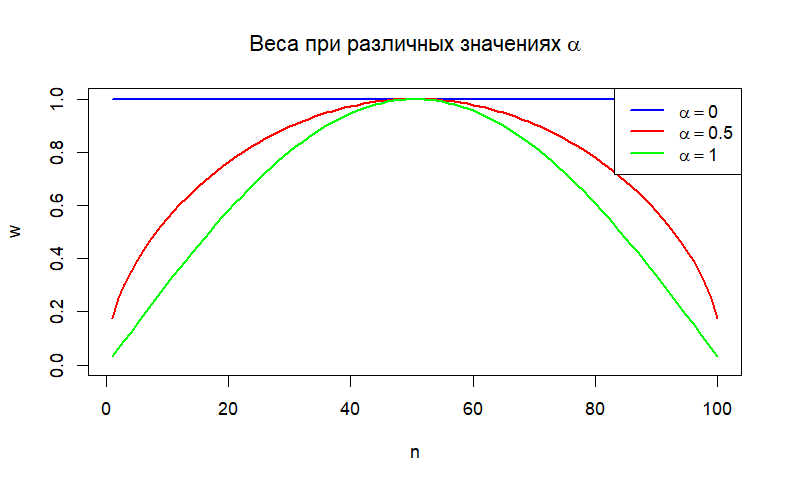
\includegraphics[width=0.5\textwidth]{../Text/img/weights.png}
		% \end{figure}

		\textbf{\structure{Шаг 1 алгорима $\GSSA$}}:

		$\mathbf{X}^{(\alpha)} = \mathcal{H}^{(\alpha)}(\TS) = [\TS_1^{\alpha} : \ldots : \TS_K^{\alpha}]$,
		$\TS_i^{(\alpha)} = ( w_1 x_{i-1}, \ldots, w_L x_{i+L-2})^{\mathrm{T}}$,
		$1 \leq i \leq K$. 
		
		\textbf{\structure{Шаги 2-4}}: аналогичны $\SSA$.
		
		\begin{comment}
			При $\alpha = 0$, $\GSSA$ --- в точности базовый алгоритм $\SSA$.
		\end{comment}

		
		% \note{
		% 	\textcolor{red}{\textbf{TODO}} 
		% 	Сослаться на статью авторов.
		% 	}
	\end{frame}
	
	
	\begin{frame}{Сравнение SSA и GSSA. Линейные фильтры 1}

		\begin{definition}
			Пусть $\TS = (\dots, x_{-1}, x_0, x_1, \dots)$ — бесконечный временной ряд. 
		
			\textbf{Линейный конечный фильтр} — оператор $\Phi$, преобразующий $\TS$ в $\TS' = (\dots, y_{-1}, y_0, y_1, \dots)$ по правилу:
			\begin{equation*}
				y_j = \sum_{i = -r_1}^{r_2} h_i x_{j-i}, \quad j \in \mathbb{Z},
			\end{equation*}
			где $r_1, r_2 \in \mathbb{N}$ — ширина фильтра, $h_i \in \mathbb{R}$ — коэффициенты.
		\end{definition}
		

		\textbf{\structure{Пример.}} При применении фильтра $\Phi$ на $\TS_{\cos} = \cos{2\pi \omega n}$, получается ряд
		$y_j = A_{\Phi}(\omega) \cos\left(2\pi\omega j + \phi_{\Phi}(\omega) \right)$.

		$\phi_{\Phi}(\omega)$ -- фазово-частотная характеристика (ФЧХ).

		$A_{\Phi}(\omega)$ -- амплитудно-частотная характеристика (АЧХ). 

		% \note{
		% 	\textcolor{red}{\textbf{TODO}} 
		% 	Пояснить, что означает АЧХ на примере.

		% 	Сказать, что будем сравнивать эти методы с точки зрения линейных фильтров.
			% }
	\end{frame}
	
	
	\begin{frame}{Сравнение SSA и GSSA. Линейные фильтры 2}
		$\TS = (x_1, \dots, x_{N})$, $(\sqrt{\lambda},\,U,\,V)$ -- собственная тройка $\SSA$. $U = (u_1, \dots, u_L)$.
		$\widetilde \TS = \mathcal{H}^{-1} ( \sqrt{\lambda} U V^T )$. 

		\textbf{\structure{Запись $\SSA$ через линейный фильтр}}:
		\begin{equation*}
			\label{eq:representation_ssa_as_filter}
			{\widetilde{x}}_{s} = \sum_{j=-(L-1)}^{L-1} \left( \sum_{k=1}^{L-|j|} u_{k} u_{k+|j|} / L \right) x_{s-j}, \quad L \leq s \leq K.
		\end{equation*}
		
		\textbf{\structure{Аналогичное представление для $\GSSA$}}:
		\begin{equation*}
			\label{eq:representation_gssa_as_filter}
			{\widetilde{x}}_{s} = \sum_{j=-(L-1)}^{L-1} \left( \sum_{k=1}^{L-|j|} u_{k}^{(\alpha)} u_{k+|j|}^{(\alpha)} w_k / \sum\limits_{i = 1}^{L}w_i \right) x_{s-j}, \quad L \leq s \leq K.
		\end{equation*}

		
		% \note{
			% \textcolor{red}{\textbf{TODO}} 
			% Убрать весь текст, оставить только представление в виде фильтров
			% }
	\end{frame}
	
	\begin{frame}{Сравнение SSA и GSSA. Пример}
		$\TS = \TS_{\sin} + \TS_{\cos} = \sin\left(\frac{2\pi}{12} n \right) + \frac{1}{2}\cos\left(\frac{2\pi}{19} n \right)$. $N = 96 \cdot 2 - 1$, $L = 48$.
		\begin{figure}[H]
			\centering
			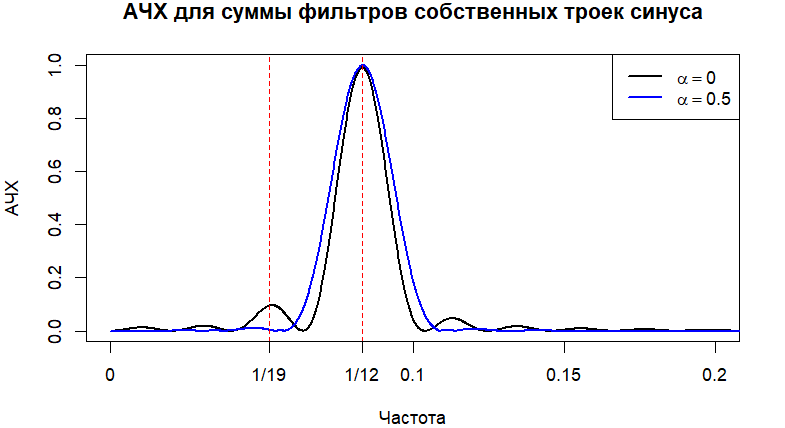
\includegraphics[width=0.8\textwidth]{../Text/img/various_alphas_sin_cos.png}
			\label{fig:various_alphas_sin_cos}
		\end{figure}
		При \(\alpha = 0.5\) АЧХ без волн, но с широкой областью около частоты синуса, что ухудшает отделение от шума, но улучшает разделение компонентов.

		% \note{
		% 	\textcolor{red}{\textbf{TODO}} 
		% 	Расписать, что $\GSSA$ хуже отделяет от шума, но лучше компоненты между собой, основываясь по рисунку. Дописать, по каким группам производилось объединение.
		% 	}
	\end{frame}
	
	
	\begin{frame}{Сравнение SSA и GSSA. Пример, продолжение}
		\begin{table}[H]
			\caption{MSE разложений $\TS = \TS_{\sin} + \TS_{\cos}$}
			\centering
			\begin{tabular}{c|ccc}
				\hline
				Метод/Ошибка & $\TS_{\sin}$ & $\TS_{\cos}$ & $\TS$ \\ 
				\hline
				$\SSA$   & 5.15e-03 & 5.15e-03 & \textbf{6.01e-30}\\ 
				$\GSSA$, $\alpha = 0.5$  & \textbf{3.68e-04} & \textbf{3.68e-04} & \textbf{9.53e-30} \\ 
				\hline
			\end{tabular}
			\label{tab:mse_ssa_gssa}
		\end{table}
		Без шума $\GSSA$ выдает результаты на порядок лучше $\SSA$.

		\begin{table}[H]
			\caption{MSE разложений $\TS = \TS_{\sin} + \TS_{\cos}+
		\varepsilon_n$, $\varepsilon_n \sim \mathrm N(0, 0.1^2)$ }
			\centering
			\begin{tabular}{c|ccc}
				\hline
				Метод & $\TS_{\sin}$ & $\TS_{\cos}$ & $\TS$ \\ 
				\hline
				$\SSA$      & 5.68e-03 & 5.44e-03 & \textbf{7.48e-04}  \\ 
				$\GSSA$, $\alpha = 0.5$ & \textbf{1.21e-03} & \textbf{1.25e-03} & 1.04e-03 \\
				\hline
			\end{tabular}
			\label{tab:errs_ssa_gssa}
		\end{table}
		
		С шумом выигрыш на порядок у $\GSSA$ пропал, но теперь $\SSA$ выделил сигнал на порядок лучше.

		% \note{
		% 	\textcolor{red}{\textbf{TODO}} 
		% 	Подтвердить этими таблицами слова из предыдущего слайда про шум и разделимость компонент.
		% }
	\end{frame}
	
	
	
	\begin{frame}{Вывод. Вложенный вариант SSA + GSSA}

		Можно объединить преимущества обоих алгоритмов, выделив сигнал с помощью $\SSA$, а затем разделив компоненты друг от друга благодаря $\GSSA$:
		\begin{table}[H]
			\label{tab:errs_ssa_gssa_united}
			\centering
			\begin{tabular}{c|ccc}
				\hline
				Метод & $\TS_{\sin}$ & $\TS_{\cos}$ & $\TS$ \\ 
				\hline
				$\SSA$ + $\GSSA$, $\alpha = 0.5$ & \textbf{1.06e-03} & \textbf{1.12e-03} & \textbf{7.15e-04} \\ 
				\hline
			\end{tabular}
		\end{table}

		Получается вложенный вариант $\SSA$.

		% \textcolor{red}{\textbf{TODO}} 
		% Дописать, что получился вложенный вариант алгоритма.
	\end{frame}
	
	
%	\begin{frame}{Метод SSA. Свойства: точная разделимость}
%		Пусть временной ряд  $\TS = \TS^{(1)} + \TS^{(2)}$ и задачей является нахождение этих слагаемых.
%		
%		Будем говорить, что ряд $\TS$ точно разделим на $\TS^{(1)} $ и $ \TS^{(2)}$, если существует такое сингулярное разложение траекторной матрицы $\mathbf X$ ряда $\TS$, что его можно разбить на две части, являющиеся сингулярными разложениями траекторных матриц рядов $\TS^{(1)}, \TS^{(2)}$ \citep{golyandina2001analysis}.
%		
%		
%		
%		
%		\note{
%			Условия точной разделимости выводятся из понятий слабо L-разделимых рядов и сильно L-разделимых рядов \citep{golyandina2001analysis}. Стоит отметить, что точная разделимость для $\cos$ достигается, если $Lw \in \mathbb{N}, \, Kw \in \mathbb{N}$, где $w$ --- частота.
%			
%			Однако условия точной разделимости достаточно жесткие и вряд ли выполнимы в реальных задачах. Тогда появляется такое понятие, как асимптотическая разделимость.
%		}
%		
%		
%	\end{frame}
%	
	
	
%	\begin{frame}{Метод SSA. Свойства: асимптотическая разделимость}
%		
%		\begin{equation*}
%			\rho_{i,j}^{(M)}=\frac{\left(\TS_{i,i+M-1}^{(1)},\TS_{j,j+M-1}^{(2)}\right)}{\left|\left|\TS_{i,i+M-1}^{(1)}\right|\right|\left|\left|\TS_{j,j+M-1}^{(2)}\right|\right|}.
%		\end{equation*}
%		
%		\begin{definition}
%			Ряды $\TS^{(1)}, \TS^{(2)}$ называются $\varepsilon$-разделимыми при длине окна $L$, если
%			\begin{equation*}
%				\rho^{(L,K)}\ {\stackrel{\mathrm{def}}{=}}\ \mathrm{max}\left(\operatorname*{max}_{1\leq i,j\leq K}|\rho_{i,j}^{(L)}|,\operatorname*{max}_{1\leq i,j\leq L}|\rho_{i,j}^{(K)}|\right)<\varepsilon
%				\text{  .}
%			\end{equation*}
%			
%		\end{definition}
%		
%		\begin{definition}
%			Если $\rho^{(L(N),K(N))} \rightarrow 0$ при некоторой последовательности $L = L(N) $, $N \rightarrow \infty$, то ряды $\TS^{(1)}, \TS^{(2)}$ называются асимптотически $L(N)$-разделимыми \citep{golyandina2001analysis}.
%		\end{definition}
%		
%		\note{
%			Для любого ряда $\TS$ длины $N$ определим
%			$\TS_{i,j}\,=\,(x_{i-1},\cdot\cdot\cdot,x_{j-1}),\;\;1\,\leq\,i\,\leq\,j\,<\,N.$
%			Пусть $\TS^{(1)}=(x_{0}^{(1)},\ldots,x_{N-1}^{(1)}),\TS^{(2)}=(x_{0}^{(2)},\ldots,x_{N-1}^{(2)}).$ Тогда определим коэффициент корреляции.
%			
%		}
		
		
%	\end{frame}
	
	
%	\begin{frame}{Метод SSA. Свойства: асимптотическая разделимость}
%		
%		
%		
%		\begin{comment}
%			Для $\SSA$ существуют алгоритмы улучшения разделимости \citep{golyandina2023intelligent}. Они позволяют более точно отделять временные ряды друг от друга. В данной работе будут использоваться методы EOSSA и FOSSA.
%		\end{comment}
%		
%		\note{
%			Для нас важно, что благодаря применению улучшения разделимости мы можем делать автоматическую группировку по заданным частотам в базовом алгоритме $\SSA$.
%		}
%		
%		
%	\end{frame}
	
	
	
	\begin{frame}{Метод CiSSA. Алгоритм}
		% Как и в $\SSA$ считается $\mathbf X$, по которой строится $\hat{\mathrm{C}}_{L}$:
		% $\hat c_m = \frac{L-m}{L}\hat{\gamma}_m + \frac{m}{L}\hat{\gamma}_{L-m}$, $ \hat{\gamma}_m = \frac{1}{N-m} \sum \limits_{t = 1}^{N-m}x_t x_{t+m}$, $ \, m = 0:L-1$.
		% \begin{equation*}
		% 	\label{eq:circ_mat}
		% 	\hat{\mathrm{C}}_{L}=\left(\begin{array}{cccc}
		% 		\hat c_{1} & \hat c_{2} & \ldots & \hat c_{L} \\
		% 		\hat c_{2} & \hat c_{1} & \ldots & \hat c_{L-1} \\
		% 		\vdots & \vdots & \vdots & \vdots \\
		% 		\hat c_{L} & \hat c_{L-1} & \hdots & \hat c_{1}
		% 	\end{array}\right).
		% \end{equation*}
		% Собственные числа и вектора матрицы $\hat{\mathrm{C}}_{L}$, задаются по формулам:
		% \begin{equation*}
		% 	\begin{split}
		% 		&U_{k}=L^{-1/2}(u_{k,1\cdot}\cdot\cdot\cdot,u_{k,L}), \, \text{где} \, 
		% 		u_{k,j}=\exp\left(-\mathrm{i}2\pi\mathrm{d}(j-1)\frac{k-1}{L}\right), \\
		% 		&\lambda_{L,k}=\sum_{m=0}^{L-1}\hat c_{m}\exp\left(i 2\pi m\frac{k-1}{L}\right), \, k = 1:L.
		% 	\end{split}
				% \end{equation*}
		\( \TS = (x_1, \ldots, x_N) \) — временной ряд.  \( 1 < L < N \) --  длина окна.
		\textbf{\structure{Алгоритм $\CISSA$}}:
		\begin{enumerate}
			\item \textbf{Построение траекторной матрицы:} как в $\SSA$.
			
			\item $l = 1:L$, ${U}_{l}=L^{-1/2}(u_{l,1},\dots,u_{l,L}), \, u_{l,j}=\exp\left(-\mathrm{i}2\pi(j-1)\frac{l-1}{L}\right).$
			\textbf{Элементарное разложение:} $w_k = \frac{k-1}{L}$, $k = 1:\lfloor \frac{L+1}{2} \rfloor$
			\begin{align*}
				&\mathbf X_{w_k}  = U_k U_k^H \mathbf X + U_{L+2-k} U_{L+2-k}^H \mathbf X;\\
				&\mathbf X_{w_{\frac{L}{2} + 1}}  = 
				U_{\frac{L}{2} + 1} U_{\frac{L}{2} + 1}^H \mathbf X, \, \text{если} \, L \mod 2 = 0,
			\end{align*}
			\textbf{Разложение:}
			$
			\mathbf{X} = \sum\limits_{k=1}^d \mathbf{X}_{w_k}, \, d = \lfloor \frac{L+1}{2} \rfloor \, (\text{или} \, \frac{L}{2} + 1).
			$

			\item \textbf{Группировка} по частотам:
			$\bigsqcup \limits_{i=1}^m I_i = 
			\bigsqcup \limits_{i=1}^m 
			\left[ w_i^{(l)}, w_i^{(r)} \right] =
			[0, 0.5]$.

			\item \textbf{Диагональное усреднение:} как в $\SSA$.
		\end{enumerate}

	\end{frame}

	\begin{frame}
		\textbf{\structure{Замечания:}}
		\bigskip
		\begin{itemize}
			\item В отличие от $\SSA$, базис подпространства которого зависит от $\TS, L, N$ (адаптивный), базис в $\CISSA$ зависит только от $L, N$ (фиксированный).
			\bigskip
			\item Поскольку группировка производится по частотам, а частоты зависят от $L$, то алгоритм применим только в случае, когда заранее известны интересующие частоты.
		\end{itemize}
	\end{frame}
	

	\begin{frame}{Метод CiSSA. Свойства: связь с разложением Фурье}
		\begin{definition}
			Разложение
			\begin{equation}
				\label{eq:fourier}
				x_n = c_0 + \sum\limits_{k = 1}^{\lfloor \frac{N+1}{2} \rfloor}\left(c_k \cos(2\pi n k / N) + s_k \sin(2\pi n k / N) \right),
			\end{equation}
			где $1 \leq n \leq N$ и $s_{N/2} = 0 $ для четного N, называется разложением Фурье ряда $\TS$. 
		\end{definition}
		\begin{comment}
			\label{comm:proector}
			Разложение Фурье -- проекции всего ряда на пространства, порожденные синусами и косинусами.
			$\CISSA$ -- разложения Фурье для $K$ векторов матрицы $\mathrm X$ +  усреднение соответствующих элементов.
		\end{comment}
		\note{
			% \textcolor{red}{\textbf{TODO}} 
			% Переписать замечание (частично сделано)

			Словами сказать, что один из вопросов моего исследования является рассмотрение того, чем cissa лучше Фурье
		}
	\end{frame}

	
	% \begin{frame}{Метод CiSSA. Свойства: нестационарный ряд}
	% 	% Для использования на нестационарных временных рядах, нужно выполнить расширения ряда (экстраполировать) \parencite{bogalo2020}.
	% 	В работе \parencite{bogalo2020} предложена модификация, улучшающая результат выделения тренда, но ухудшающая разделение периодических компонент:		
	% 	\begin{figure}[htbp]
	% 		\centering
	% 		\begin{subfigure}[b]{0.49\textwidth} % Первая картинка
	% 			\includegraphics[width=\textwidth]{../Text/img/extended_IP_values.png}
	% 		\end{subfigure}
	% 		\hfill % Добавляет горизонтальный отступ между картинками
	% 		\begin{subfigure}[b]{0.49\textwidth} % Вторая картинка
	% 			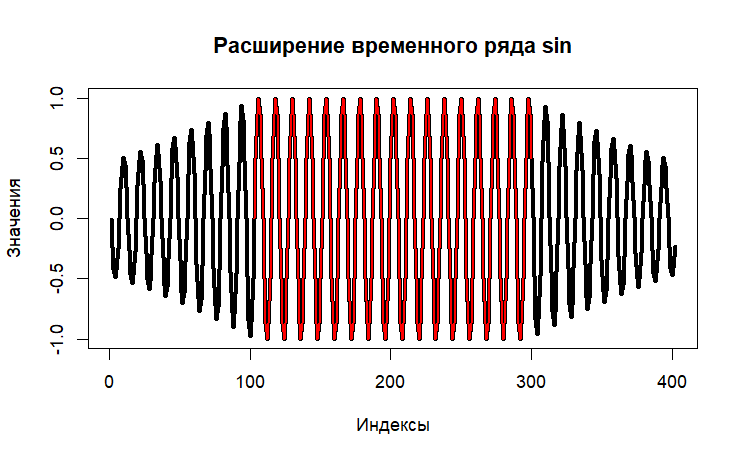
\includegraphics[width=\textwidth]{../Text/img/extended_sin.png}
	% 		\end{subfigure}
	% 		\caption{Красный -- настоящий ряд, черный -- его расширение}
	% 	\end{figure}

	% 	Таким образом, можно использовать алгоритм на нестационарных рядах.
		
		
	% 	\note{
	% 		\textcolor{red}{\textbf{TODO}} 
	% 		Написать алгоритм расширения ряда в конце как приложение в конце. сказать, что изначально алгоритм пригоден только для стационарных рядов.
	% 	}
	% \end{frame}
	
		
	
	\begin{frame}{Сравнение SSA, Фурье, CiSSA. Точная разделимость}
		Фиксируем временной ряд $\TS = \TS_{1} + \TS_{2} =$ $= A_1 \cos(2\pi w_1 n + \varphi_1) + A_2 \cos(2\pi w_2 n + \varphi_2)$.
		\newline \newline
		Условия точной разделимости $\TS$ для разложения Фурье: \\
		$Nw_1, Nw_2 \in \mathbb{N}$, $w_1 \not = w_2$.
		
		Условия точной разделимости $\TS$ для $\CISSA$: \\
		$Lw_1, Lw_2 \in \mathbb{N}$, $w_1 \not = w_2$.
		
		Условия точной разделимости $\TS$ для $\SSA$: \\
		$Lw_1, Lw_2, Kw_1, Kw_2 \in \mathbb{N}$, $w_1 \not = w_2$, $A_1 \not = A_2$.
		\newline \newline
		Таким образом, условия на разделение косинусов, слабее у методов $\CISSA$ и Фурье, чем у $\SSA$.
	\end{frame}
	
	\begin{frame}{Пример. Точная разделимость}
		\textbf{\structure{Пример: }}
		$\TS = \TS_{\sin} + \TS_{\cos} = A_1 \sin(2\pi w_1 n ) + A_2 \cos(2\pi w_2 n ) $
		
		\begin{table}[ht]
			\centering
			\resizebox{0.95\textwidth}{!}{ % Масштабируем таблицу
			\begin{tabular}{l|l|lll}
				\hline
				\textbf{Метод} & \textbf{Параметры} & $\MSE\left(\TS_{\sin}\right)$ & $\MSE\left(\TS_{\cos}\right)$ & $\MSE\left(\TS\right)$ \\ 
				\hline
				SSA & \( Lw \in \mathbb{N}, Kw \in \mathbb{N} \), \( A_1 \neq A_2 \) & \textbf{6.8e-30} & \textbf{1.5e-29} & \textbf{1.8e-29} \\ 
				SSA EOSSA & \( Lw \in \mathbb{N}, Kw \in \mathbb{N} \), \( A_1 \neq A_2 \), \( r = 4 \) & \textbf{8.2e-30} & \textbf{6.5e-30} & \textbf{5.5e-30} \\ 
				Fourier & \( Nw \in \mathbb{N} \) & \textbf{3.4e-28} & \textbf{9.8e-29} & \textbf{4.0e-28} \\ 
				CiSSA & \( Lw \in \mathbb{N} \), \( A_1 \neq A_2 \) & \textbf{1.1e-29} & \textbf{6.5e-30} & \textbf{7.8e-30} \\ 
				\hline
				SSA & \( Lw \in \mathbb{N}, Kw \in \mathbb{N} \), \( A_1 = A_2 \) & 3.8e-04 & 3.8e-04 & \textbf{6.0e-29} \\ 
				SSA & \( Lw \in \mathbb{N} \), \( Kw \notin \mathbb{N} \), \( A_1 = A_2 \) & 4.9e-03 & 3.4e-03 & \textbf{5.9e-29} \\ 
				Fourier & \( Nw \notin \mathbb{N} \) & 7.6e-03 & 3.3e-03 & 5.6e-03 \\ 
				SSA EOSSA & \( Lw \in \mathbb{N} \), \( Kw \notin \mathbb{N} \), \( A_1 = A_2 \), \( r = 4 \) & \textbf{1.4e-29} & \textbf{2.9e-29} & \textbf{1.1e-29} \\ 
				\hline
			\end{tabular}
			}
		\end{table}
		По таблице видно, что при нарушении условий точной разделимости, результаты значительно ухудшаются. При этом, EOSSA исправляет ситуацию.

		\note{
			Длину N ряда сложно подбирать, поэтому будем рассматривать случаи, когда N хорошее и плохое. А L всегда можем изменить, поэтому все L подобраны наилучшим образом. $w_1$, $w_2$ фиксированы
		}
	\end{frame}
	

	\begin{frame}{Сравнение SSA, Фурье, CiSSA. Асимптотическая разделимость}
		Асимптотически разделимы в методе $\SSA$ полиномы, гармонические функции \parencite{golyandina2001analysis}.
		
		В алгоритме разложения $\CISSA$ (Фурье) увеличение длины окна $L$ ($N$) изменяет сетку частот. Это означает, что даже если не удастся подобрать такое $L$ ($N$), при котором косинус будет точно отделим, его постепенное увеличение позволит приблизить частоты сетки к частоте компоненты. В итоге, можно снизить ошибку выделения нужной компоненты, учитывая соседние частоты.

		\note{
			\textcolor{red}{\textbf{TODO}} 
			Переформулировать с меньшим количеством слов (тяжело)
		}
	\end{frame}



	\begin{frame}{Пример. Асимптотическая разделимость}
		\textbf{\structure{Пример: }}
		$\TS = \TS_{e\cdot\sin} + \TS_{e\cdot\cos} = e^{A_1 n } \sin(2\pi w_1 n ) + e^{A_2 n} \cos(2\pi w_2 n ) $.

		\begin{table}[ht]
			\centering
			\resizebox{0.95\textwidth}{!}{ % Масштабируем таблицу
			\begin{tabular}{l|l|lll}
				\hline
				\textbf{Метод} & \textbf{Параметры} & $\MSE\left(\TS_{e \cdot \sin}\right)$ & $\MSE\left(\TS_{e \cdot \cos}\right)$ & $\MSE\left(\TS\right)$ \\ 
				\hline
				SSA & \( Lw \in \mathbb{N}, Kw \in \mathbb{N} \) & 5.3e-05 & 5.3e-05 & \textbf{1.2e-27} \\ 
				SSA EOSSA & \( Lw \in \mathbb{N}, Kw \in \mathbb{N}, r = 4 \) & \textbf{3.0e-28} & \textbf{4.4e-28} & \textbf{7.4e-29} \\ 
				Fourier & \( Nw \in \mathbb{N} \) & 6.7e-02 & 1.4e-02 & 4.9e-02 \\ 
				CiSSA & \( Lw \in \mathbb{N} \) & 2.6e-02 & 3.8e-03 & 1.5e-02 \\ 
				\hline
				SSA & \( Lw \in \mathbb{N}, Kw \notin \mathbb{N} \) & 4.8e-04 & 4.8e-04 & \textbf{1.1e-27} \\ 
				Fourier & \( Nw \notin \mathbb{N} \) & 1.1e-01 & 3.7e-02 & 1.1e-01 \\ 
				SSA EOSSA & \( Lw \in \mathbb{N}, Kw \notin \mathbb{N}, r = 4 \) & \textbf{2.8e-28} & \textbf{4.2e-28} & \textbf{7.5e-29} \\ 
				\hline
			\end{tabular}
			}
		\end{table}

		При домножении на экспоненты периодик, все результаты ухудшились кроме EOSSA. Фурье и $\CISSA$ значительно ухудшились в точности разделения.
	\end{frame}


	\begin{frame}{Пример 1. Отделение сигнала от шума}
		\textbf{\structure{Пример 1: }}
		$\TS = \TS_{\sin} + \TS_{\cos} + \TS_{\mathrm{Noise}} =$ $ = A_1 \sin(2\pi w_1 n ) + A_2 \cos(2\pi w_2 n ) + \varepsilon_n$, $\varepsilon \sim \mathrm N(0, 0.1^2) $
		\begin{table}[ht]
			\centering
			\resizebox{0.95\textwidth}{!}{ % Масштабируем таблицу
			\begin{tabular}{l|l|lll}
				\hline
				\textbf{Метод} & \textbf{Параметры} & $\MSE\left(\TS_{\sin}\right)$ & $\MSE\left(\TS_{\cos}\right)$ & $\MSE\left(\TS\right)$ \\ 
				\hline
				SSA & \( Lw \in \mathbb{N}, Kw \in \mathbb{N} \) & 2.7e-04 & 3.3e-04 & 6.0e-04 \\ 
				SSA EOSSA & \( Lw \in \mathbb{N}, Kw \in \mathbb{N} \) & 2.7e-04 & 3.3e-04 & 6.0e-04 \\ 
				Fourier & \( Nw \in \mathbb{N} \) & 1.5e-04 & 2.1e-04 & 3.6e-04 \\ 
				CiSSA & \( Lw \in \mathbb{N} \) & 1.6e-04 & 2.8e-04 & 4.3e-04 \\ 
				\hline
				SSA & \( Lw \in \mathbb{N}, Kw \in \mathbb{N}, A_1 = A_2 \) & 2.5e-04 & 3.3e-04 & 6.0e-04 \\ 
				SSA & \( Lw \in \mathbb{N}, Kw \notin \mathbb{N}, A_1 = A_2 \) & 4.9e-03 & 3.4e-03 & 6.0e-04 \\ 
				Fourier & \( Nw \notin \mathbb{N} \) & 2.6e-02 & 7.3e-02 & 9.8e-02 \\ 
				SSA EOSSA & \( Lw \in \mathbb{N}, Kw \notin \mathbb{N}, A_1 = A_2 \) & 2.7e-04 & 3.4e-04 & 6.0e-04 \\ 
				\hline
			\end{tabular}
			}
		\end{table}
		Фурье значительно хуже остальных выделил сигнал.
	\end{frame}

	\begin{frame}{Пример 2. Отделение сигнала от шума}
		\textbf{\structure{Пример 2: }}
		$\TS = \TS_{e\cdot\sin} + \TS_{e\cdot\cos} + \TS_{\mathrm{Noise}}= $ $=e^{A_1 n } \sin(2\pi w_1 n ) + e^{A_2 n} \cos(2\pi w_2 n ) + \varepsilon_n$, $\varepsilon \sim \mathrm N(0, 0.1^2) $
		\begin{table}[ht]
			\centering
			\resizebox{1\textwidth}{!}{ % Масштабируем таблицу
			\begin{tabular}{l|l|lll}
				\hline
				\textbf{Метод} & \textbf{Параметры} & $\MSE\left(\TS_{e \cdot \sin}\right)$ & $\MSE\left(\TS_{e \cdot \cos}\right)$ & $\MSE\left(\TS\right)$ \\ 
				\hline
				SSA & \( Lw \in \mathbb{N}, Kw \in \mathbb{N} \) & 3.1e-04 & 3.6e-04 & 5.6e-04 \\ 
				SSA EOSSA & \( Lw \in \mathbb{N}, Kw \in \mathbb{N} \) & 2.2e-04 & 3.4e-04 & 5.6e-04 \\ 
				Fourier & \( Nw \in \mathbb{N} \) & 1.1e-01 & 1.3e+00 & 1.4e+00 \\ 
				CiSSA & \( Lw \in \mathbb{N} \) & 2.8e-02 & 3.8e-01 & 4.0e-01 \\ 
				\hline
			\end{tabular}
			}
			\caption{Example Table} 
		\end{table}
		Фурье совсем плохо себя показал. $\CISSA$ ухудшил результаты в сравнении с тем, что было без шума.
	\end{frame}
	
	
	
	% \begin{frame}{Сравнение SSA, Фурье, CiSSA. Выводы 1}
		
	% 	\begin{table}[H]
	% 		\centering
	% 		\begin{center}
	% 			\resizebox{0.95\textwidth}{!}{ % Масштабируем таблицу
	% 			\begin{tabular}{l|cccccccc}
	% 				\hline
	% 				Метод/Условие  & $\cos$,                 & $\cos$,                    & $\cos$,                     & $\TS_{\mathrm{np1}}$   & $\TS_{\mathrm{np}}$ & group\\ 
	% 				& $Lw \in \mathbb N$, & $Lw\in \mathbb N$,    & $Lw \not\in \mathbb N$, &             \\
	% 				& $Kw\in \mathbb N$  & $Kw \not\in \mathbb N$ & $Kw \not\in \mathbb N$  &             \\ 
	% 				\hline
	% 				SSA            & $+$                     & $\to$                      & $\to$                       & $\to$ & $\to$ & $-$ \\
	% 				SSA EOSSA      & $+$                     & $\to$                      & $\to$                       & $\to$ & $\to$ & $+$ \\
	% 				CiSSA          & $+$                     & $+$                        & $\to$                       & $-$   & $-$ & $+$ \\
	% 				CiSSA extended & $+$                     & $+$                        & $\to$                       & $\to$ & $-$ & $+$ \\
	% 				\hline
	% 			\end{tabular}
	% 		}
	% 		\end{center}
	% 		\caption{Преимущества и недостатки методов $\SSA$, $\CISSA$} 
	% 		\label{tab:advantages_ssa_cissa}
	% 	\end{table}
		
	% 	\begin{table}[H]
	% 		\centering
	% 		\begin{center}
	% 			\resizebox{0.95\textwidth}{!}{ % Масштабируем таблицу
	% 			\begin{tabular}{l|cccccccc}
	% 				\hline
	% 				Метод/Условие  & cos,                 & cos,                  & $\TS_{\mathrm{np1}}$   & $\TS_{\mathrm{np}}$ & group\\ 
	% 				& $Nw \in \mathbb N$ & $Nw \not \in \mathbb N$ \\
	% 				\hline
	% 				Fourier                           & $+$                        & $\to$                       & $-$   & $-$ & $+$ \\
	% 				Fourier extended                         & $+$                        & $\to$                       & $\to$   & $-$ & $+$ \\
	% 				\hline
	% 			\end{tabular}
	% 		}
	% 		\end{center}
	% 		\caption{Преимущества и недостатки методов Fourier} 
	% 		\label{tab:advantages_fourier}
	% 	\end{table}
	% \end{frame}
	
	
	\begin{frame}{Сравнение SSA, Фурье, CiSSA. Выводы 2}
		По полученным результатам, можно следующие выводы: 
		\begin{enumerate}
			\item $\CISSA$ и разложение Фурье работает лучше базового $\SSA$ только в том случае, когда периодики имеют одинаковые амплитуды. При этом, $\SSA$ с EOSSA исправляет этот недостаток. Во всех остальных случаях $\CISSA$ и разложение Фурье показывают результаты не лучше $\SSA$. 
			\item $\CISSA$ показывает себя лучше Фурье.
			\item $\CISSA$ при добавлении шума и отклонении от своих показывает значительное ухудшение в разделении сигнала и компонент между собой.
		\end{enumerate}

		% \note{
		% 	\textcolor{red}{\textbf{TODO}} 
		% 	Переписать выводы в соответствии с примерами.
		% }
	\end{frame}
	
	
	\begin{frame}[allowframebreaks]{Список литературы}
		\small
		% \bibliographystyle{plain}
		% \bibliography{ref}
		\printbibliography
	\end{frame}

	
\end{document}
